\section{ISDB-Tb}
\label{sec:isdbtb}

ISDB-Tb (\textit{Integrated Services Digital Broadcasting -- Terrestrial, Brazilian version}) es la norma de televisión digital terrestre que Argentina adoptó en 2009 para la Televisión Digital Abierta \cite{decreto1148}. Toma la capa física de la norma japonesa ISDB-T (ARIB STD-B31) \cite{arib_b31}, recogida por la UIT en la Recomendación BT.1306 \cite{itu_bt1306}, con las modificaciones brasileñas de la norma ABNT NBR 15601 \cite{abnt15601}:
\begin{itemize}
    \item Compresión de video H.264 / MPEG-4 AVC, en lugar de MPEG-2.
    \item Audio AAC.
    \item Middleware de interactividad Ginga.
    \item Canales de $6 \, [MHz]$.
\end{itemize}

\subsection{Principio de funcionamiento de OFDM}
OFDM (\textit{Orthogonal Frequency Division Multiplexing}) divide el flujo de datos en miles de subflujos lentos, cada uno de los cuales modula una subportadora distinta. Las subportadoras están separadas exactamente $\Delta f = 1/T_u$, la inversa de la duración útil del símbolo. Con esa separación son ortogonales: en el centro del espectro de cada una, las demás pasan por cero (\autoref{fig:ofdm}), de modo que se solapan sin interferirse. La modulación y la demodulación se hacen con la transformada rápida de Fourier (IFFT en el transmisor, FFT en el receptor).

\begin{figure}[H]
    \centering
    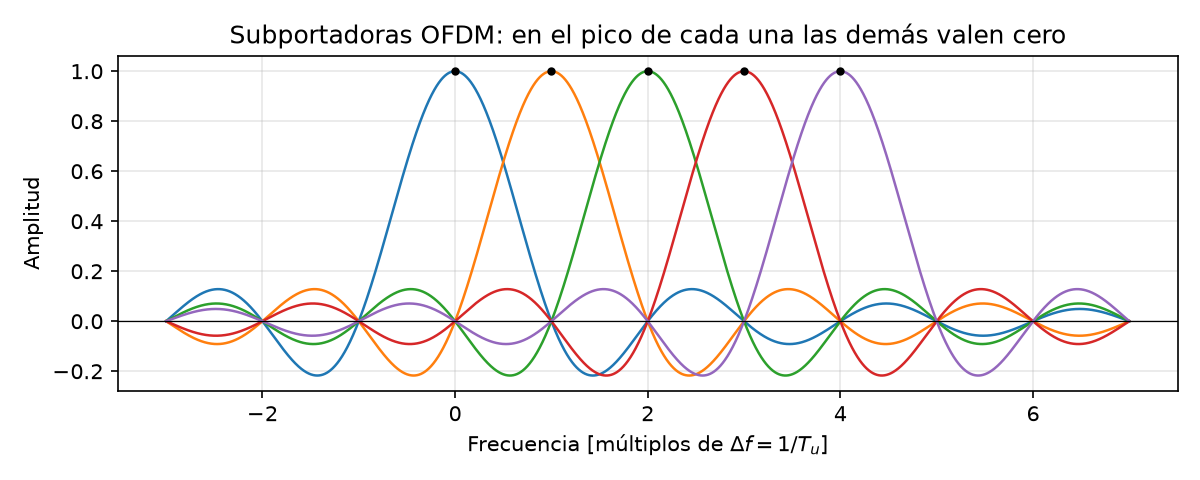
\includegraphics[width=0.8\textwidth]{teoria/ofdm_subportadoras.png}
    \caption{Espectros de las subportadoras OFDM: cada una tiene su máximo donde las demás se anulan (esquema propio).}
    \label{fig:ofdm}
\end{figure}

La ventaja frente a una portadora única es la robustez al multitrayecto. Cada símbolo OFDM dura cientos de microsegundos, mucho más que el retardo de los ecos. Además, a cada símbolo se le antepone un intervalo de guarda $T_g$, una copia de su parte final, de duración $1/4$, $1/8$, $1/16$ o $1/32$ de $T_u$. Si los ecos llegan dentro del intervalo de guarda no producen interferencia entre símbolos, y el efecto de cada eco sobre cada subportadora se reduce a un cambio de amplitud y de fase, que el receptor corrige con las portadoras piloto. Esto también permite las redes de frecuencia única (SFN), en las que varios transmisores emiten el mismo canal en la misma frecuencia.

ISDB-Tb tiene tres modos, que difieren en el tamaño de la FFT (\autoref{tab:modos}). Los modos con más subportadoras tienen símbolos más largos y toleran ecos más largos, pero son más sensibles al efecto Doppler en la recepción móvil.

\begin{table}[H]
    \centering
    \caption{Modos de transmisión de ISDB-Tb en canales de $6 \, [MHz]$ \cite{arib_b31, abnt15601}.}
    \label{tab:modos}
    \begin{tabular}{c c c c c c}
        \toprule
        \textbf{Modo} & \textbf{FFT} & \textbf{Subportadoras} & \textbf{Por segmento} & \textbf{$\Delta f$ [kHz]} & \textbf{$T_u$ [µs]} \\
        \midrule
        1 & 2k & 1.405 & 108 & $3{,}968$ & $252$ \\
        2 & 4k & 2.809 & 216 & $1{,}984$ & $504$ \\
        3 & 8k & 5.617 & 432 & $0{,}992$ & $1.008$ \\
        \bottomrule
    \end{tabular}
\end{table}

\subsection{Organización del canal en segmentos}
El ancho útil se divide en 13 segmentos OFDM de $6/14 \, [MHz] = 428{,}57 \, [kHz]$ cada uno, que en total ocupan $5{,}57 \, [MHz]$ del canal de $6 \, [MHz]$ (\autoref{fig:isdbtb_segmentos}). Cada segmento tiene subportadoras de datos, pilotos dispersos para estimar el canal y portadoras de control:
\begin{itemize}
    \item \underline{TMCC}: llevan la configuración de la transmisión (modulación, tasa de código y cantidad de segmentos de cada capa), de modo que el receptor se configura solo.
    \item \underline{AC}: llevan información auxiliar, como las alertas de emergencia EWBS.
\end{itemize}
Los segmentos se numeran del 0 al 12 desde el centro del canal hacia afuera. El segmento 0 ocupa el centro, lo que permite que un receptor de banda angosta decodifique solo ese segmento.

\begin{figure}[H]
    \centering
    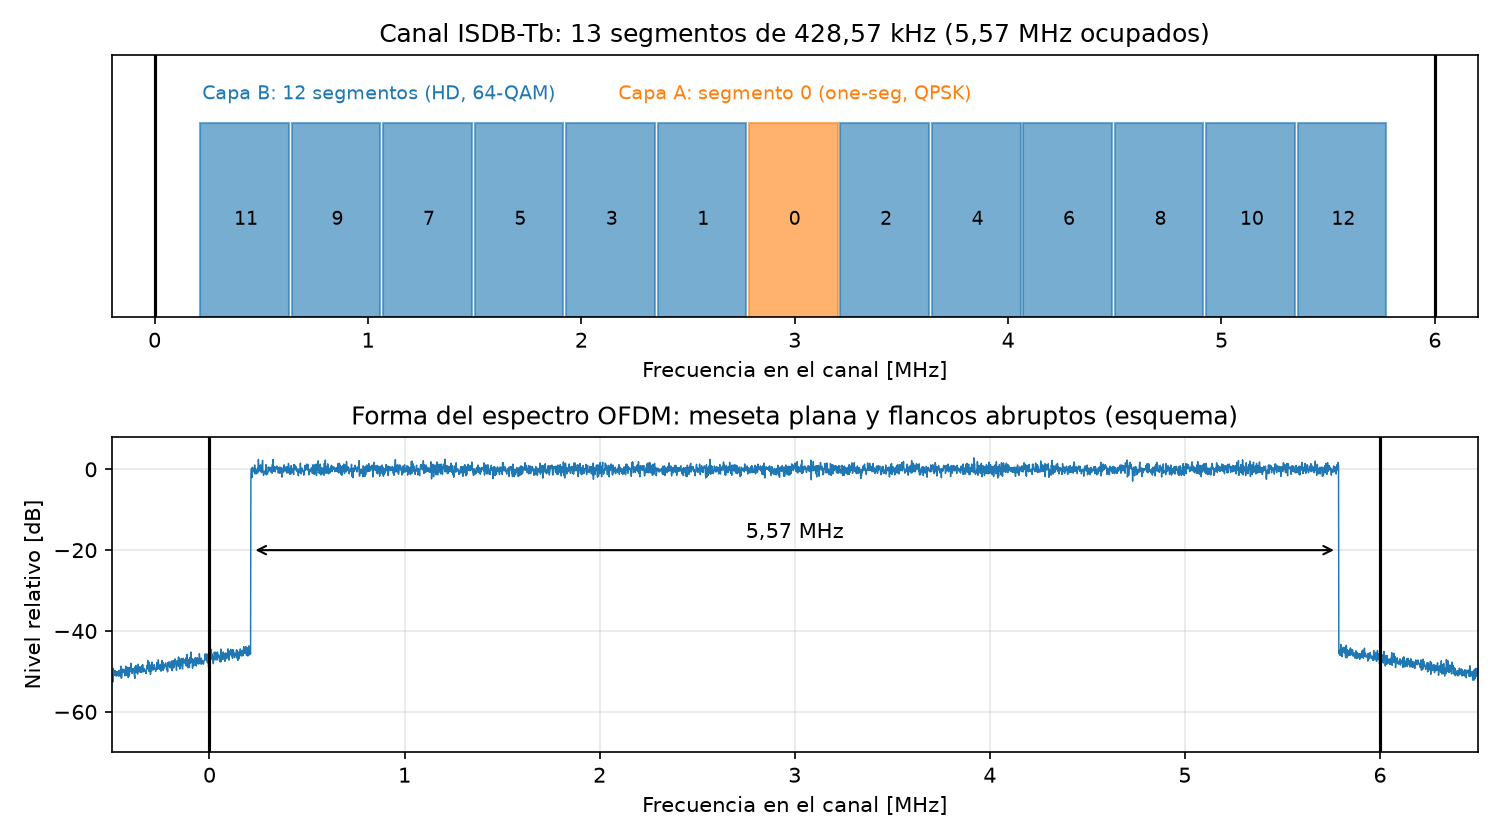
\includegraphics[width=\textwidth]{teoria/isdbtb_segmentos.png}
    \caption{Organización del canal ISDB-Tb en 13 segmentos con la configuración típica de dos capas, y forma del espectro OFDM (esquemas propios).}
    \label{fig:isdbtb_segmentos}
\end{figure}

\subsection{Distintos servicios en un mismo canal}
Los 13 segmentos se agrupan en hasta tres capas jerárquicas (A, B y C), cada una con su propia modulación, tasa de código del código convolucional interno ($1/2$, $2/3$, $3/4$, $5/6$ o $7/8$) y profundidad de entrelazado temporal. Las modulaciones posibles son DQPSK, QPSK, 16-QAM y 64-QAM. Cada capa transporta su propio flujo de transporte, con uno o varios programas.

La configuración más usada en la TDA es de dos capas:
\begin{itemize}
    \item \underline{Capa A:} el segmento central (\textit{one-seg}), con QPSK y tasa de código $2/3$, para receptores portátiles y teléfonos.
    \item \underline{Capa B:} los otros 12 segmentos, con 64-QAM y tasa $3/4$, para un programa en alta definición o varios en definición estándar para recepción fija.
\end{itemize}
Así, una sola emisora transmite al mismo tiempo, en la misma frecuencia, el programa en HD y su versión para dispositivos móviles. Otras combinaciones permiten, por ejemplo, tres capas o varios programas SD en la capa B (multiprogramación).

\subsection{Recepción fija y móvil}
\begin{itemize}
    \item \underline{Recepción fija:} con antena exterior directiva, a una altura de unos $10 \, [m]$, el receptor tiene buena relación señal a ruido y un canal estable. Se pueden usar modulaciones densas, como 64-QAM con tasa de código alta, que maximizan la capacidad.
    \item \underline{Recepción móvil y portátil:} antenas pequeñas a nivel del suelo, dentro de edificios o en vehículos. El receptor tiene menor señal, multitrayecto intenso y variaciones rápidas del canal por efecto Doppler, y necesita modulaciones robustas, como QPSK con tasa $1/2$ o $2/3$, entrelazado temporal largo y, a veces, un modo con menos subportadoras.
\end{itemize}
El \textit{one-seg} es la solución de ISDB para la recepción móvil: al ocupar solo $430 \, [kHz]$, el receptor consume menos y puede integrarse en un teléfono.

\subsection{Configuración, capacidad y robustez}
La capacidad de una capa es proporcional a la cantidad de segmentos, a los bits por símbolo, a la tasa de código y al factor de guarda. Para un segmento en el modo 1, con 96 subportadoras de datos:
\begin{equation}
    R_{seg} = \frac{96 \cdot \log_2 M \cdot r \cdot \frac{188}{204}}{T_u\,(1 + T_g/T_u)}
    \label{eq:tasa_segmento}
\end{equation}
El resultado no depende del modo, porque al duplicar las subportadoras se duplica la duración del símbolo. Por ejemplo, con 64-QAM, $r = 3/4$ e intervalo de guarda $1/8$:
\begin{equation}
    R_{seg} = \frac{96 \cdot 6 \cdot 0{,}75 \cdot 0{,}922}{252 \, [\mu s] \cdot 1{,}125} = 1{,}40 \, [Mbps]
\end{equation}
y los 12 segmentos de la capa B dan $16{,}8 \, [Mbps]$, suficientes para un programa HD y uno SD en H.264. La capa A con QPSK y $r = 2/3$ aporta $0{,}42 \, [Mbps]$. Según la configuración, el canal completo ofrece entre $3{,}65 \, [Mbps]$ (DQPSK, $r = 1/2$, guarda $1/4$) y $23{,}2 \, [Mbps]$ (64-QAM, $r = 7/8$, guarda $1/32$).

Cada aumento de capacidad se paga con robustez: pasar de QPSK a 64-QAM triplica los bits por símbolo, pero exige unos $12 \, [dB]$ más de relación señal a ruido. Una tasa de código más alta tiene menos redundancia para corregir errores, y un intervalo de guarda más corto tolera ecos más cortos y limita el tamaño de una SFN. La configuración se elige según el servicio y el área de cobertura que se quiere alcanzar.
